\chapter{Introduction}

Proteins are essential to modern day life,
performing machine-like transformations of chemicals as enzymes,
provide structural support and move cells,
transportation and communication,
and antigen recognition.
In fact, proteins are so important for the function of life that their blueprints are written in our DNA\cite{avery_studies_1944} using a near-universal encoding\cite{crick_origin_1968,hinegardner_rationale_1963},
providing evidence for the theory that all life on Earth shares common ancestry\cite{darwin_origin_1859}.

Understanding how proteins work can be undertaken using a variety of strategies, including genetic analysis \cite{lander_initial_2001}, but one of the most informative has been to determine structures, as knowing what a machine looks like can provide insight into its functionality.
We have been able to determine the structures of proteins at a high resolution since the first published structures, of myoglobin and hemoglobin(\cite{kendrew_three-dimensional_1958,perutz_structure_1960}.
Still, there are many more known protein sequences in the universe of life than exist known structures in available databases of experimentally determined structures (88,032,926 unique sequences vs. 123,153 known structures, as of Aug. 12, 2017 \cite{berman_protein_2000,noauthor_uniprot:_2017}).
We can turn to the power of computation to help determine protein structures when no experimental data exists.

\section{Why computation is hard}

\begin{wrapfigure}{L}{0.5\textwidth}
  \centering
  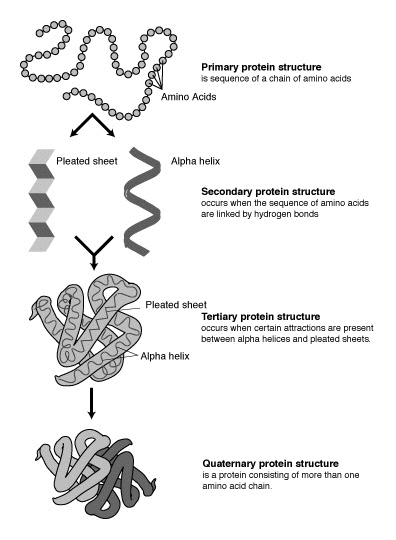
\includegraphics[width=0.48\textwidth,keepaspectratio]{figures/protein-structure.png}
  \caption[Protein sequence/structure]{Knowledge of the primary amino acid sequence is a common input for computational structure prediction programs, which then can produce possible models of the protein's secondary, tertiary, and quaternary structure. Figure produced by: U.S. National Institutes of Health.}
  \label{fig:protein-structure}
  \vspace{-12pt}
\end{wrapfigure}

Protein structure prediction can operate on the ``primary'', ``secondary'', ``tertiary'', or ``quaternary'' levels (\cref{fig:protein-structure}).
And while modern protein secondary structure prediction methods can achieve relatively high accuracies (of about 80\%\cite{pirovano_protein_2009}), protein structure prediction of more detailed models remains a major challenge.

The difficulty of computational protein structure prediction can be thought of as two complementary challenges: the ``sampling'' problem and the ``scoring'' problem.

\paragraph{Sampling}
sampling is tough, yo.

Some of the first computational methods for protein structure prediction focused on ab-initio folding (TODO cite), or predicting the three-dimensional structure of a protein from its amino acid code.

Sampling/scoring
Levinthal paradoc
This all leads into representation question

Although there are so many proteins, not as many protein folds (cite number of protein folds).

Increasing computing power can be relied on (TODO cite Moore's law) to allow more and more detailed representations of protein structure in computer programs, ranging from coarse-grained representations of beads (TODO cite something where one residue is the point), to methods that simulate every atom in proteins (TODO cite first all-atom representations), to quantum (TODO cite) and methods beyond our current understanding of physics.

Choosing a representation that encodes the desired features of proteins to tackle a certain problem is an important consideration before starting to tackle these problems.
Perturbing protein structures via design allows for the functionality of existing proteins to be altered(TODO cite enzyme design original papers), and entirely new functionalities (TODO cite enzyme design) and structures (TODO cite top7) to be created.
Validiating that the representation used is general enough to be effective for the desired use case is an important consideration of computational methodologies.

Fragments, coupled moves, other ways to sample effectively (including starting at known strcture (TODO cite scaffold design)).

\section{what i did}
Although proteins tend to ``fold'' around a single state (TODO cite) that represents the most stable conformation (with some exceptions (TODO cite kinetic trap)), life takes place at non-frozen, biological temperatures, causing proteins to take on multiple states (TODO cite).
Some of this inherent noise of life (entropy) is actually essential to life itself (TODO cite what is life).

Recognizing that proteins take on multiple conformations allows for a more complex computational representation that has proven valuable (TODO cite).

I set out to utilize our current level of protein tools (TODO cite some tools) to generate biosensors.
I also wanted to rigourously test the performance of methods, providing a foundation to build up to these more complex representations.

Representing proteins as dynamic has allowed better results of predicting interactions, allowing us to study biological systems (TODO cite mavor) and further change how proteins interact via stabilizing or detablizing mutations.


\section{conclusions}

Rosetta software has provided multiple effective representations of protein structures (TODO cite centroid, all atom) that have enabled powerful applications in structure prediction and design.

Further advancements have been made here in ensuring that software is reliable and useful to the community, in addition to showing how new advances in scoring have helped our lab's sampling protocols.

We can now (with more powerful computers) use more complex, ensemble-based representation of protein structures, and learn new things about biology.